% Enhanced Nerdfit dynamics visualization with improved layout
% Compile: pdflatex model-equations-enhanced.tex
\documentclass[border=20pt]{standalone}

\usepackage{lmodern}
\usepackage{amsmath,amssymb}
\usepackage{xcolor}
\usepackage{tikz}
\usetikzlibrary{arrows.meta,positioning,calc,shadows,backgrounds,fit}

\newcommand{\ind}{\mathbf{1}}

% --- Phenomenon palette ---
\definecolor{st}{HTML}{1B2631}      % state variables
\definecolor{hb}{HTML}{1B7F6A}      % habit & automaticity
\definecolor{mv}{HTML}{C45C26}      % motivation & reward
\definecolor{ef}{HTML}{5C4D8A}      % effort / opportunity cost
\definecolor{ex}{HTML}{6B4C9A}      % expectation excess & calibration
\definecolor{id}{HTML}{2874A6}      % identity & self-concept
\definecolor{cx}{HTML}{7D6608}      % behavioral complexity
\definecolor{fn}{HTML}{AF601A}      % fantasy / indulgence
\definecolor{cl}{HTML}{B03A2E}      % collapse & disinhibition
\definecolor{ct}{HTML}{1F618D}      % context
\definecolor{mt}{HTML}{566573}      % meta-control

% Color macros
\newcommand{\St}[1]{\ensuremath{\textcolor{st}{\mathbf{#1}}}}
\newcommand{\Hb}[1]{\ensuremath{\textcolor{hb}{#1}}}
\newcommand{\Mv}[1]{\ensuremath{\textcolor{mv}{#1}}}
\newcommand{\Ef}[1]{\ensuremath{\textcolor{ef}{#1}}}
\newcommand{\Ex}[1]{\ensuremath{\textcolor{ex}{#1}}}
\newcommand{\Id}[1]{\ensuremath{\textcolor{id}{#1}}}
\newcommand{\Cx}[1]{\ensuremath{\textcolor{cx}{#1}}}
\newcommand{\Fn}[1]{\ensuremath{\textcolor{fn}{#1}}}
\newcommand{\Cl}[1]{\ensuremath{\textcolor{cl}{#1}}}
\newcommand{\Mt}[1]{\ensuremath{\textcolor{mt}{#1}}}
\newcommand{\Ct}[1]{\ensuremath{\textcolor{ct}{\text{#1}}}}
\newcommand{\Ctii}{\ensuremath{\textcolor{ct}{\mathit{ii}}}}

% Card style
\tikzset{
  equation card/.style={
    draw=black!30,
    line width=1.5pt,
    rounded corners=8pt,
    fill=white,
    drop shadow={shadow xshift=3pt, shadow yshift=-3pt, opacity=0.3}
  },
  legend box/.style={
    draw=black!20,
    rounded corners=4pt,
    fill=black!5,
    inner sep=8pt
  },
  phenomenon tag/.style={
    rounded corners=2pt,
    inner sep=3pt,
    font=\tiny\sf\bfseries,
    text=white
  }
}

\newcommand{\phenomenontag}[2]{%
  \tikz[baseline=(tag.base)]\node[phenomenon tag, fill=#1](tag){#2};%
}

\begin{document}

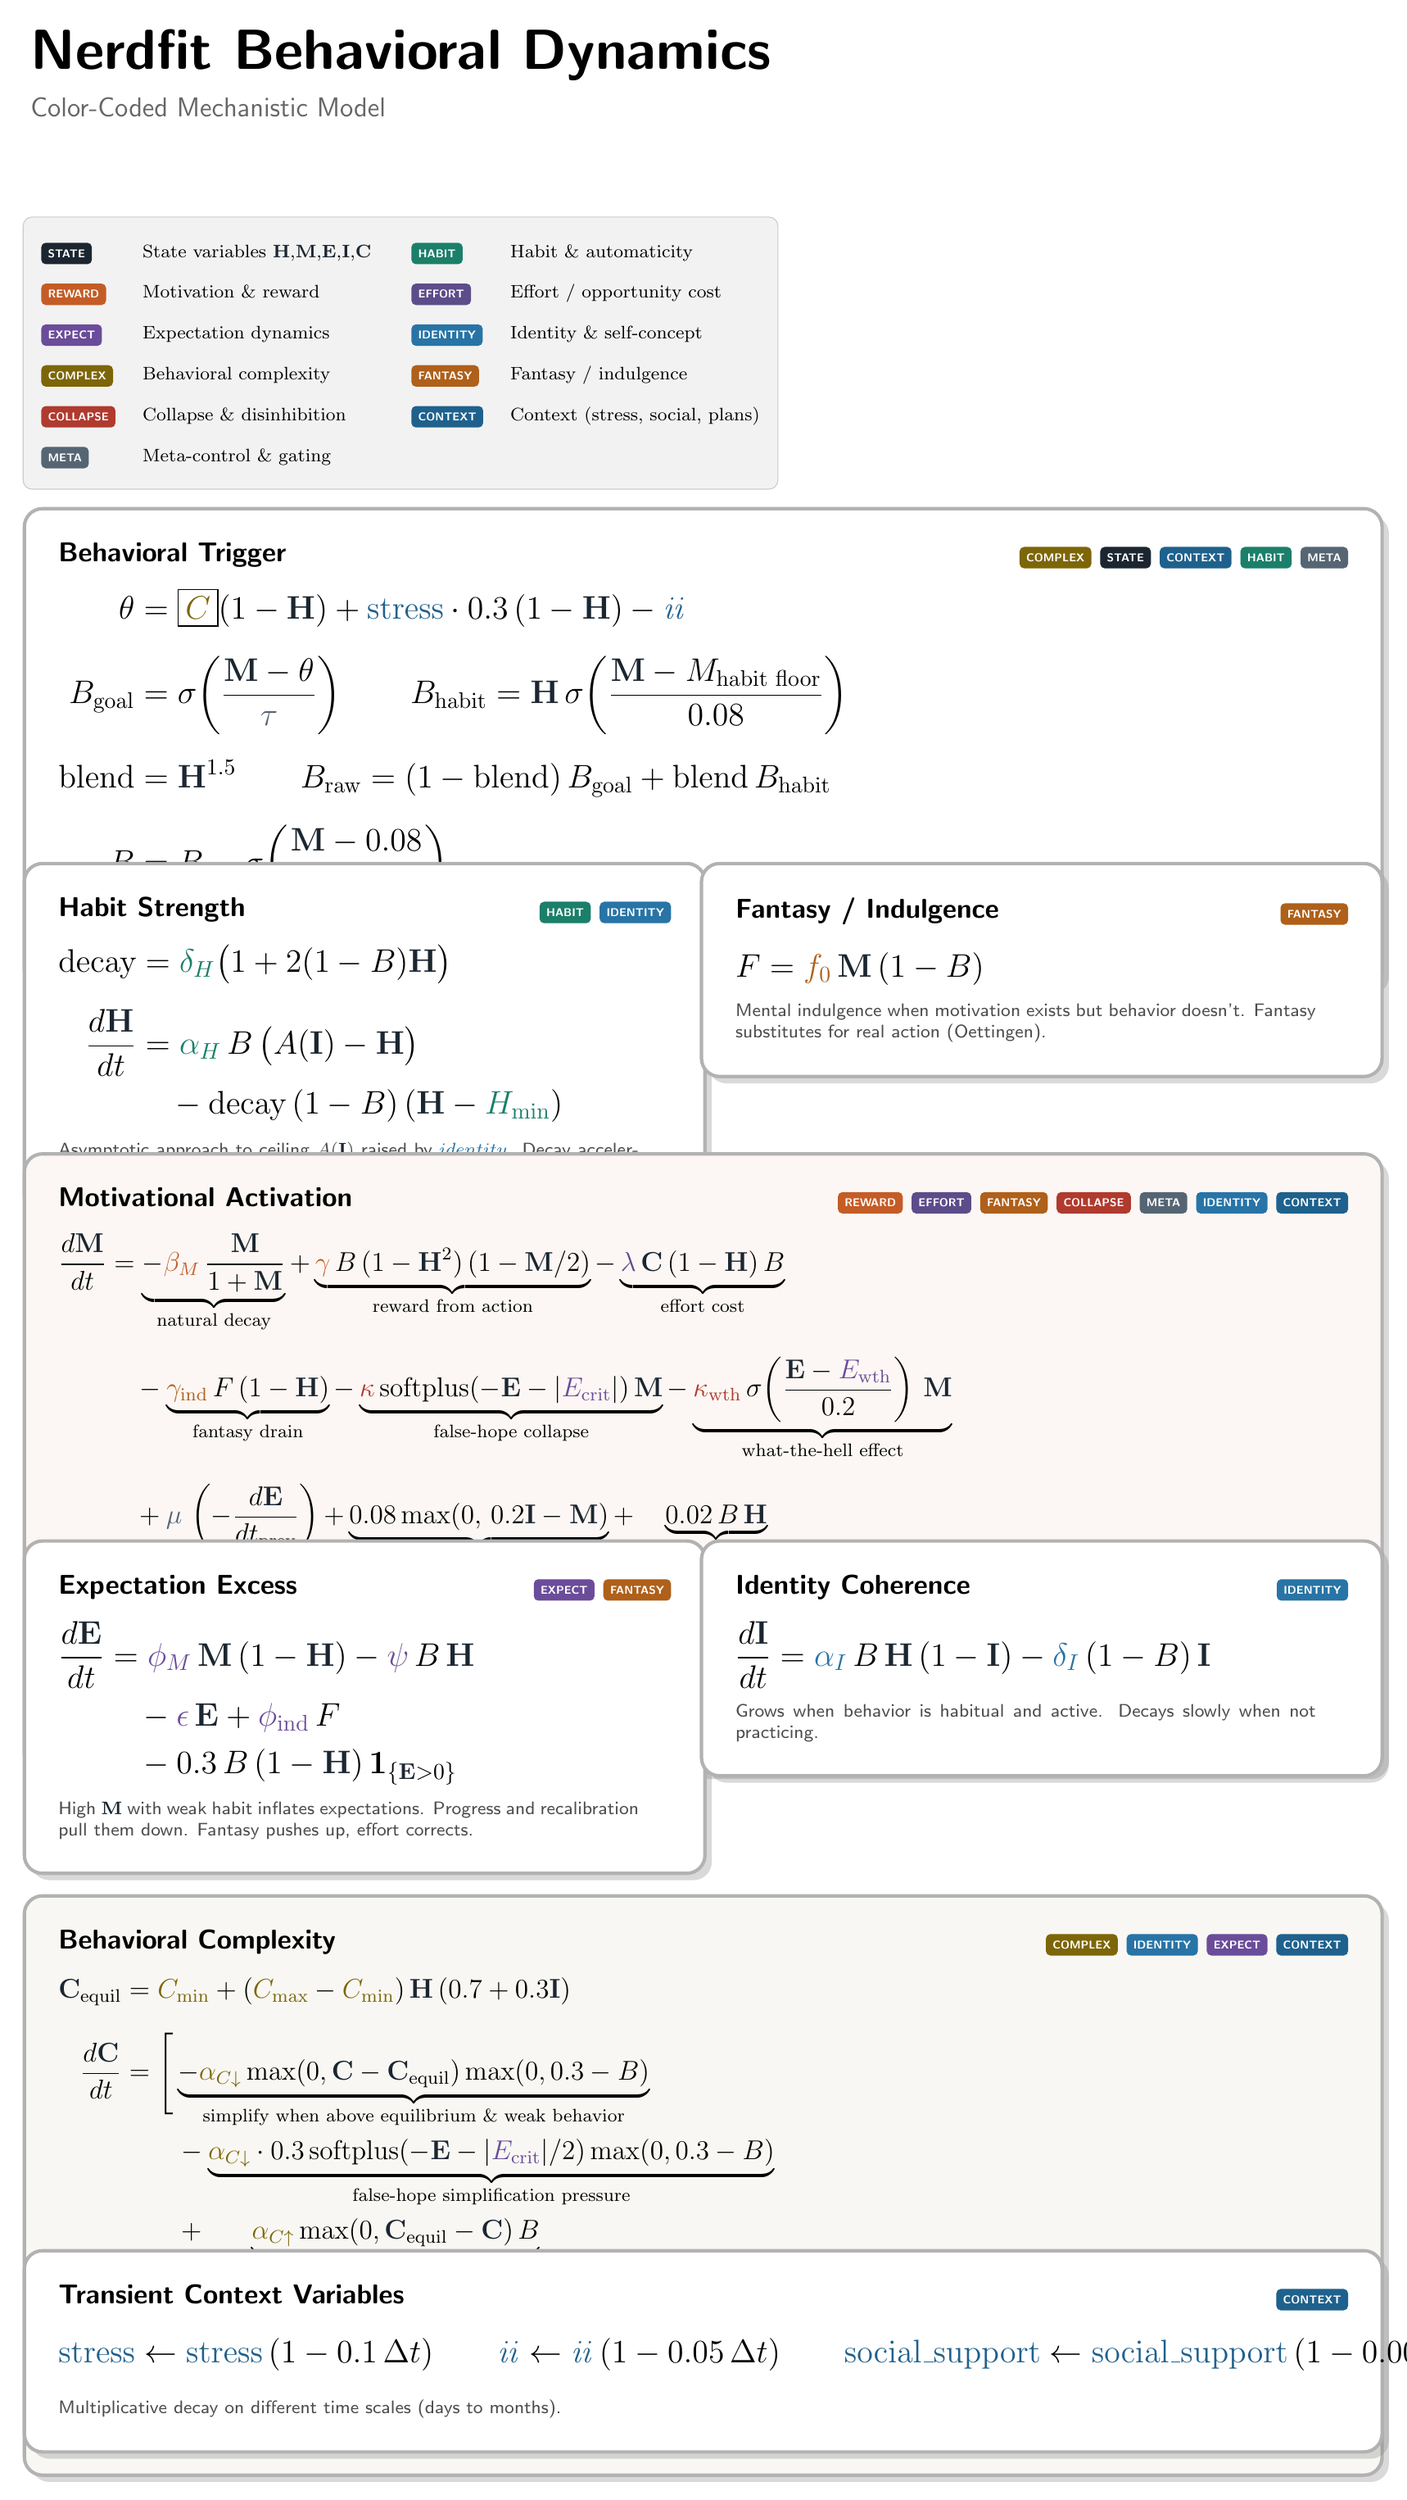
\begin{tikzpicture}[font=\large]

  % Title
  \node[font=\Huge\sffamily\bfseries, anchor=west] at (0,0) {Nerdfit Behavioral Dynamics};
  \node[font=\large\sffamily, anchor=west, text=black!60] at (0,-0.8) {Color-Coded Mechanistic Model};

  % Legend
  \begin{scope}[shift={(0,-2.5)}]
    \node[legend box, anchor=north west] (legend) at (0,0) {
      \begin{tabular}{@{}ll@{\hspace{1.5em}}ll@{}}
        \phenomenontag{st}{STATE} & \footnotesize State variables \St{H},\St{M},\St{E},\St{I},\St{C} &
        \phenomenontag{hb}{HABIT} & \footnotesize Habit \& automaticity \\[4pt]
        \phenomenontag{mv}{REWARD} & \footnotesize Motivation \& reward &
        \phenomenontag{ef}{EFFORT} & \footnotesize Effort / opportunity cost \\[4pt]
        \phenomenontag{ex}{EXPECT} & \footnotesize Expectation dynamics &
        \phenomenontag{id}{IDENTITY} & \footnotesize Identity \& self-concept \\[4pt]
        \phenomenontag{cx}{COMPLEX} & \footnotesize Behavioral complexity &
        \phenomenontag{fn}{FANTASY} & \footnotesize Fantasy / indulgence \\[4pt]
        \phenomenontag{cl}{COLLAPSE} & \footnotesize Collapse \& disinhibition &
        \phenomenontag{ct}{CONTEXT} & \footnotesize Context (stress, social, plans) \\[4pt]
        \phenomenontag{mt}{META} & \footnotesize Meta-control \& gating &
      \end{tabular}
    };
  \end{scope}

  % Main equations - arranged in grid
  \begin{scope}[shift={(0,-7)}]

    % Row 1: Behavioral trigger
    \node[equation card, anchor=north west, inner sep=15pt] (trigger) at (0,0) {
      \begin{minipage}{20cm}
        \textbf{\large\sffamily Behavioral Trigger}\hfill
        \phenomenontag{cx}{COMPLEX}
        \phenomenontag{st}{STATE}
        \phenomenontag{ct}{CONTEXT}
        \phenomenontag{hb}{HABIT}
        \phenomenontag{mt}{META}

        \vspace{8pt}
        \Large
        $\displaystyle
        \begin{aligned}
          \theta &= \boxed{\Cx{C}}(1-\St{H}) + \Ct{stress}\cdot 0.3\,(1-\St{H}) - \Ctii \\[0.5em]
          B_{\text{goal}} &= \sigma\!\left(\frac{\St{M}-\theta}{\Mt{\tau}}\right)
          \qquad
          B_{\text{habit}} = \St{H}\,\sigma\!\left(\frac{\St{M}-M_{\text{habit floor}}}{0.08}\right) \\[0.5em]
          \text{blend} &= \St{H}^{1.5}
          \qquad
          B_{\text{raw}} = (1-\text{blend})\,B_{\text{goal}} + \text{blend}\,B_{\text{habit}} \\[0.5em]
          B &= B_{\text{raw}}\,\sigma\!\left(\frac{\St{M}-0.08}{0.03}\right)
        \end{aligned}
        $

        \vspace{6pt}
        \begin{minipage}{19cm}
          \footnotesize\sffamily\color{black!70}
          Complexity \Cx{C} and stress raise the threshold; implementation intentions lower it.
          As habit strength \St{H} grows, control shifts from motivation-vs-threshold to automatic drive.
        \end{minipage}
      \end{minipage}
    };

    % Row 2: Habit and Fantasy
    \begin{scope}[shift={(0,-5.5)}]
      \node[equation card, anchor=north west, inner sep=15pt] (habit) at (0,0) {
        \begin{minipage}{9.5cm}
          \textbf{\large\sffamily Habit Strength}\hfill
          \phenomenontag{hb}{HABIT}
          \phenomenontag{id}{IDENTITY}

          \vspace{8pt}
          \Large
          $\displaystyle
          \begin{aligned}
            \text{decay} &= \Hb{\delta_H}\bigl(1 + 2(1-B)\St{H}\bigr) \\[0.5em]
            \frac{d\St{H}}{dt} &= \Hb{\alpha_H}\,B\,\bigl(A(\St{I})-\St{H}\bigr) \\
            &\quad - \text{decay}\,(1-B)\,(\St{H}-\Hb{H_{\min}})
          \end{aligned}
          $

          \vspace{6pt}
          \begin{minipage}{9cm}
            \footnotesize\sffamily\color{black!70}
            Asymptotic approach to ceiling $A(\St{I})$ raised by \Id{identity}.
            Decay accelerates when not practicing.
          \end{minipage}
        \end{minipage}
      };

      \node[equation card, anchor=north west, inner sep=15pt] (fantasy) at (10.5,0) {
        \begin{minipage}{9.5cm}
          \textbf{\large\sffamily Fantasy / Indulgence}\hfill
          \phenomenontag{fn}{FANTASY}

          \vspace{8pt}
          \Large
          $\displaystyle
          F = \Fn{f_0}\,\St{M}\,(1-B)
          $

          \vspace{6pt}
          \begin{minipage}{9cm}
            \footnotesize\sffamily\color{black!70}
            Mental indulgence when motivation exists but behavior doesn't.
            Fantasy substitutes for real action (Oettingen).
          \end{minipage}
        \end{minipage}
      };
    \end{scope}

    % Row 3: Motivation (large)
    \begin{scope}[shift={(0,-10)}]
      \node[equation card, anchor=north west, inner sep=15pt, fill=mv!5] (motivation) at (0,0) {
        \begin{minipage}{20cm}
          \textbf{\large\sffamily Motivational Activation}\hfill
          \phenomenontag{mv}{REWARD}
          \phenomenontag{ef}{EFFORT}
          \phenomenontag{fn}{FANTASY}
          \phenomenontag{cl}{COLLAPSE}
          \phenomenontag{mt}{META}
          \phenomenontag{id}{IDENTITY}
          \phenomenontag{ct}{CONTEXT}

          \vspace{8pt}
          \large
          $\displaystyle
          \begin{aligned}
            \frac{d\St{M}}{dt} &=
              \underbrace{-\Mv{\beta_M}\,\frac{\St{M}}{1+\St{M}}}_{\text{natural decay}}
              + \underbrace{\Mv{\gamma}\,B\,(1-\St{H}^2)\,(1-\St{M}/2)}_{\text{reward from action}}
              - \underbrace{\Ef{\lambda}\,\St{C}\,(1-\St{H})\,B}_{\text{effort cost}} \\[0.6em]
              &\quad - \underbrace{\Fn{\gamma_{\text{ind}}}\,F\,(1-\St{H})}_{\text{fantasy drain}}
              - \underbrace{\Cl{\kappa}\,\mathrm{softplus}(-\St{E}-|\Ex{E_{\text{crit}}}|)\,\St{M}}_{\text{false-hope collapse}}
              - \underbrace{\Cl{\kappa_{\text{wth}}}\,\sigma\!\left(\frac{\St{E}-\Ex{E_{\text{wth}}}}{0.2}\right)\,\St{M}}_{\text{what-the-hell effect}} \\[0.6em]
              &\quad + \underbrace{\Mt{\mu}\,\left(-\frac{d\St{E}}{dt_{\text{prev}}}\right)}_{\text{velocity feedback}}
              + \underbrace{0.08\max(0,\,0.2\St{I}-\St{M})}_{\text{identity nudge}}
              + \underbrace{0.02\,B\,\St{H}}_{\text{habit maintenance}} \\[0.6em]
              &\quad - \underbrace{0.3\,\Ct{stress}\,\St{M}\,(1-\St{H})\,(1-0.3\,\Ct{social})}_{\text{stress drain}}
              + \underbrace{0.05\max(0,\,0.15\,\Ct{social}-\St{M})}_{\text{social support}}
              + \underbrace{\max(0,-d\St{C}/dt)\cdot 0.3}_{\text{simplification boost}}
          \end{aligned}
          $

          \vspace{6pt}
          \begin{minipage}{19.5cm}
            \footnotesize\sffamily\color{black!70}
            Central hub: reward from action before habit saturates, effort cost scaled by complexity.
            Indulgence and expectation collapses drain \St{M}. Meta-control velocity feedback.
            Identity and habit provide sustenance. Stress and social context modulate the balance.
          \end{minipage}
        \end{minipage}
      };
    \end{scope}

    % Row 4: Expectation and Identity
    \begin{scope}[shift={(0,-16)}]
      \node[equation card, anchor=north west, inner sep=15pt] (expectation) at (0,0) {
        \begin{minipage}{9.5cm}
          \textbf{\large\sffamily Expectation Excess}\hfill
          \phenomenontag{ex}{EXPECT}
          \phenomenontag{fn}{FANTASY}

          \vspace{8pt}
          \Large
          $\displaystyle
          \begin{aligned}
            \frac{d\St{E}}{dt} &=
              \Ex{\phi_M}\,\St{M}\,(1-\St{H})
              - \Ex{\psi}\,B\,\St{H} \\
              &\quad - \Ex{\epsilon}\,\St{E}
              + \Ex{\phi_{\text{ind}}}\,F \\
              &\quad - 0.3\,B\,(1-\St{H})\,\ind_{\{\St{E}>0\}}
          \end{aligned}
          $

          \vspace{6pt}
          \begin{minipage}{9cm}
            \footnotesize\sffamily\color{black!70}
            High \St{M} with weak habit inflates expectations.
            Progress and recalibration pull them down.
            Fantasy pushes up, effort corrects.
          \end{minipage}
        \end{minipage}
      };

      \node[equation card, anchor=north west, inner sep=15pt] (identity) at (10.5,0) {
        \begin{minipage}{9.5cm}
          \textbf{\large\sffamily Identity Coherence}\hfill
          \phenomenontag{id}{IDENTITY}

          \vspace{8pt}
          \Large
          $\displaystyle
          \frac{d\St{I}}{dt} =
            \Id{\alpha_I}\,B\,\St{H}\,(1-\St{I})
            - \Id{\delta_I}\,(1-B)\,\St{I}
          $

          \vspace{6pt}
          \begin{minipage}{9cm}
            \footnotesize\sffamily\color{black!70}
            Grows when behavior is habitual and active.
            Decays slowly when not practicing.
          \end{minipage}
        \end{minipage}
      };
    \end{scope}

    % Row 5: Complexity
    \begin{scope}[shift={(0,-21.5)}]
      \node[equation card, anchor=north west, inner sep=15pt, fill=cx!5] (complexity) at (0,0) {
        \begin{minipage}{20cm}
          \textbf{\large\sffamily Behavioral Complexity}\hfill
          \phenomenontag{cx}{COMPLEX}
          \phenomenontag{id}{IDENTITY}
          \phenomenontag{ex}{EXPECT}
          \phenomenontag{ct}{CONTEXT}

          \vspace{8pt}
          \large
          $\displaystyle
          \begin{aligned}
            \St{C}_{\text{equil}} &= \Cx{C_{\min}} + (\Cx{C_{\max}}-\Cx{C_{\min}})\,\St{H}\,(0.7+0.3\St{I}) \\[0.6em]
            \frac{d\St{C}}{dt} &= \Bigg[
              \underbrace{-\Cx{\alpha_{C\downarrow}}\max(0,\St{C}-\St{C}_{\text{equil}})\max(0,0.3-B)}_{\text{simplify when above equilibrium \& weak behavior}} \\
              &\quad\quad - \underbrace{\Cx{\alpha_{C\downarrow}}\cdot 0.3\,\mathrm{softplus}\!\left(-\St{E}-|\Ex{E_{\text{crit}}}|/2\right)\max(0,0.3-B)}_{\text{false-hope simplification pressure}} \\
              &\quad\quad + \underbrace{\Cx{\alpha_{C\uparrow}}\max(0,\St{C}_{\text{equil}}-\St{C})\,B}_{\text{progressive overload when below equilibrium}} \\
              &\quad\quad + \underbrace{\Cx{\alpha_{C\uparrow}}\cdot 0.3\,\St{I}\max(0,\St{H}-0.3)\max(0,\St{C}_{\text{equil}}-\St{C})}_{\text{identity-driven complexity growth}}
            \Bigg]\,(1+\Ct{social\_support})
          \end{aligned}
          $

          \vspace{6pt}
          \begin{minipage}{19.5cm}
            \footnotesize\sffamily\color{black!70}
            Equilibrium complexity rises with habit and identity.
            Progressive overload when performing; simplification when overwhelmed.
            Social support scales adaptation rate.
          \end{minipage}
        \end{minipage}
      };
    \end{scope}

    % Row 6: Context decay
    \begin{scope}[shift={(0,-27)}]
      \node[equation card, anchor=north west, inner sep=15pt] (context) at (0,0) {
        \begin{minipage}{20cm}
          \textbf{\large\sffamily Transient Context Variables}\hfill
          \phenomenontag{ct}{CONTEXT}

          \vspace{8pt}
          \Large
          $\displaystyle
          \begin{aligned}
            \Ct{stress} &\gets \Ct{stress}\,(1-0.1\,\Delta t)
            \qquad
            \Ctii \gets \Ctii\,(1-0.05\,\Delta t)
            \qquad
            \Ct{social\_support} \gets \Ct{social\_support}\,(1-0.003\,\Delta t)
          \end{aligned}
          $

          \vspace{6pt}
          \begin{minipage}{19cm}
            \footnotesize\sffamily\color{black!70}
            Multiplicative decay on different time scales (days to months).
          \end{minipage}
        \end{minipage}
      };
    \end{scope}

  \end{scope}

\end{tikzpicture}

\end{document}
